\chapter{Problem Identification and Resolution}


\section{Issue in network connection}

During the connecting process listed in section~\ref{subsec:5g-network}, it was found that the router had been misconfigured prior to the test.
As a result, the actual LAN was a 5G network, while the built-in Wi-Fi module only supports 2.4G~\cite{arduino_nina_w10_datasheet}.
This was revealed by running an example sketch that scans for all available networks that the Arduino can join.
After that, the unsuccessful LAN was replaced with a cellular network provided by an iPhone, where the Arduino was able to recognize and connect.

%-----------This is a FIGURE-----------------------
\begin{figure}[htbp]
	\centering
	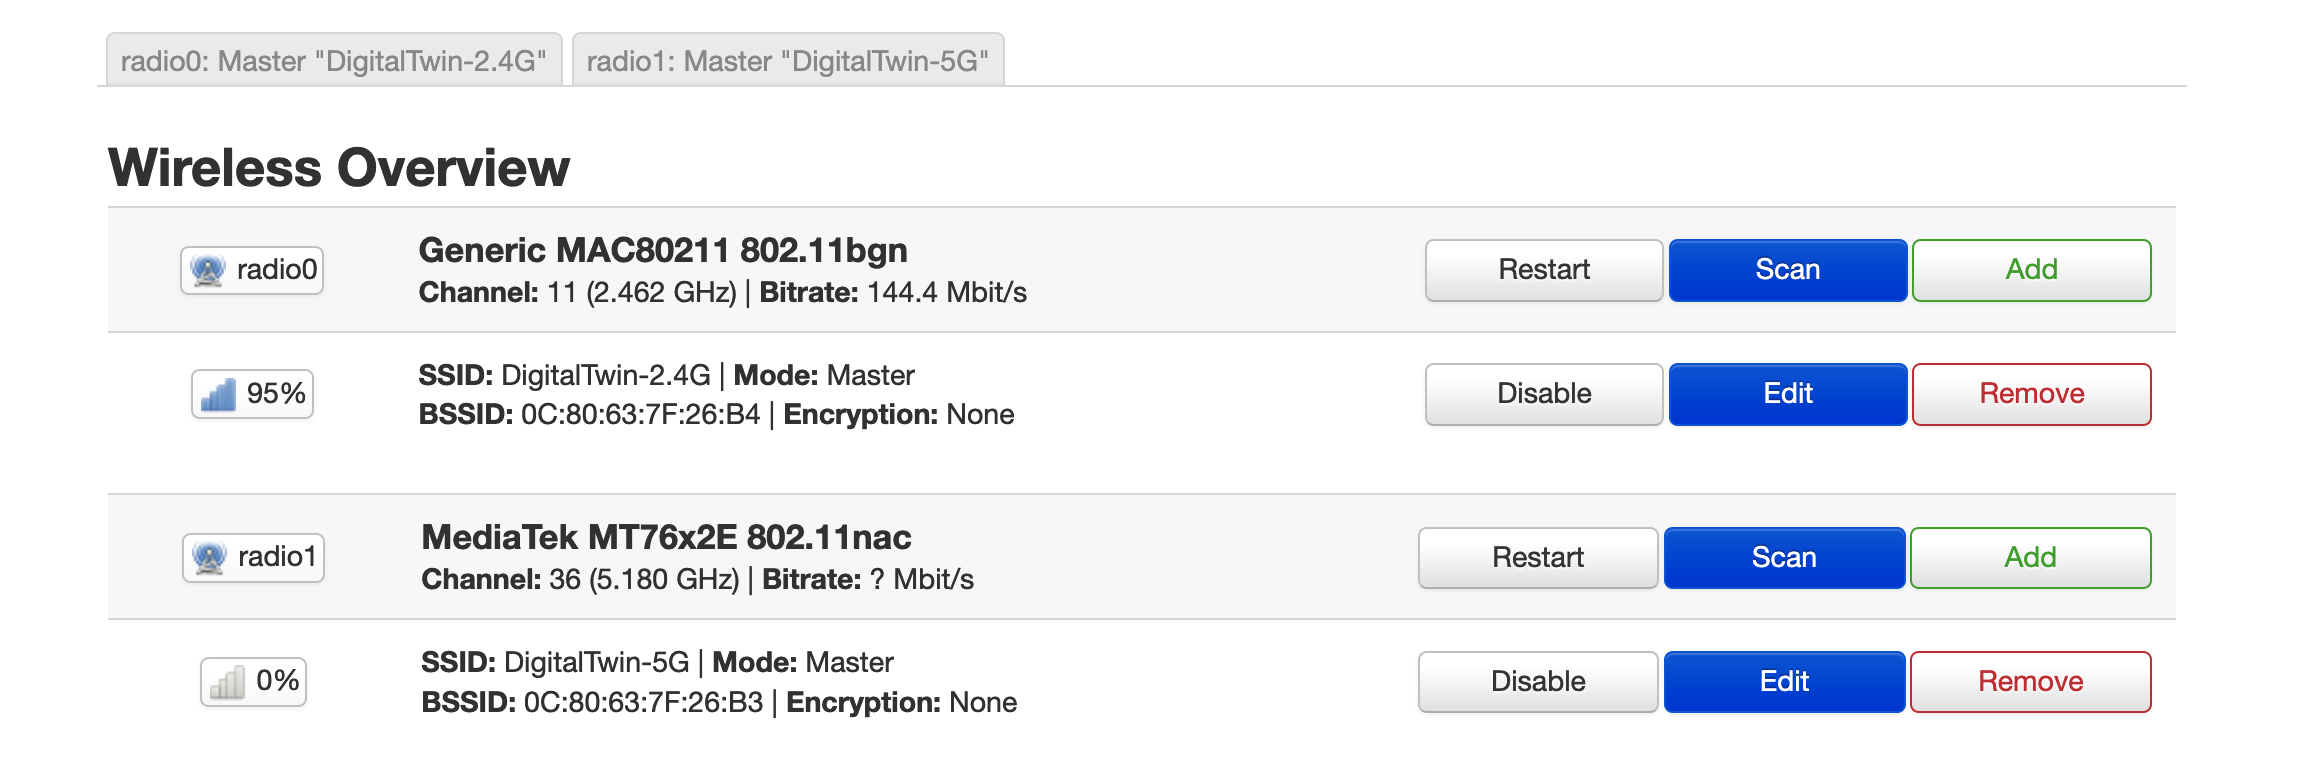
\includegraphics[width=0.8\textwidth]{
		fileForWriting/config}
	\caption[Revised configuration of router]{Revised configuration of router to provide a 2.4G network named ``DigitalTwin-2.4G''.}
	\label{fig:config-5G}
\end{figure}
%--------End of this FIGURE -----------

Such comparison highlighted that the module was working where the router configuration may be improper.
By checking existed configurations and switching the 5G network to 2.4G shown in Figure~\ref{fig:config-5G}, the network provided by the router was eventually recognized and connected by Arduino.

%-----------This is a FIGURE-----------------------
\begin{figure}[htbp]
	\centering
	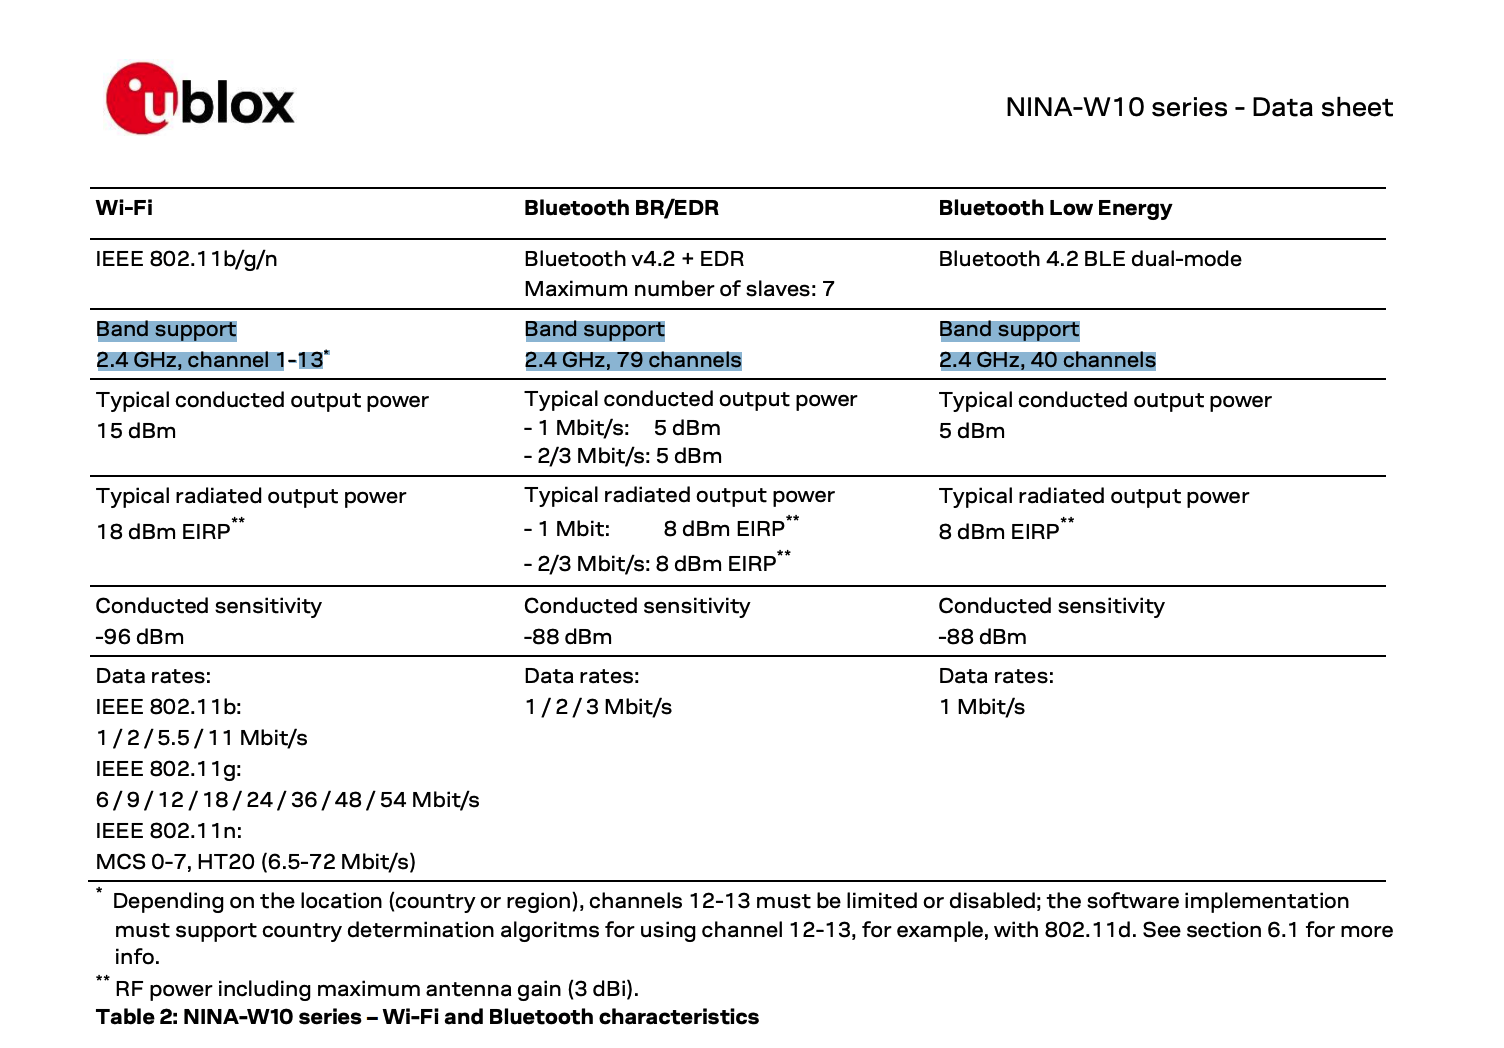
\includegraphics[width=\textwidth]{
		fileForWriting/wifinina}
	\caption[Datasheet of the onboard Wi-Fi module ``NINA-W10'']{Datasheet of the onboard Wi-Fi module ``NINA-W10'', indicating that it only supports the 2.4GHz frequency band.}
	\label{fig:2.4Gonly}
\end{figure}
%--------End of this FIGURE -----------


\section{Issue of ``no socket available''}
\subsection{Problem locating}
During the integration phase, a huge issue was encountered: the Arduino could only send motion data to the server for a very short time (from seconds to at most 3 minutes), where then the built-in Wi-Fi module would throw an error called ``no socket available''.

Although the IMU module and wireless transmission module had passed their own stress tests, an additional stress test for the new framework was subsequently conducted, which involved sending const string messages.
During the test, the Arduino was able to send a const char array continuously without any issues for half hour.
Such stability indicated that the new code framework was not the cause of the problem.

With these three stress tests, this unstable output was eventually identified as ``a function incompatibility between the IMU components and the onboard Wi-Fi component''.


\subsection{Problem analyzing}
Further researching revealed that even though the Wi-Fi module communicates with MCU using SPI protocol, it also has another channel for IIC communication as portrayed in  Figure~\ref{fig:IIC-conflict}.
Such ``additional'' IIC channel is then connected to external IIC channel between the IMU components and MCU\@.
This may have implications for the result of ``no socket available''.

%-----------This is a FIGURE-----------------------
\begin{figure}[htbp]
	\centering
	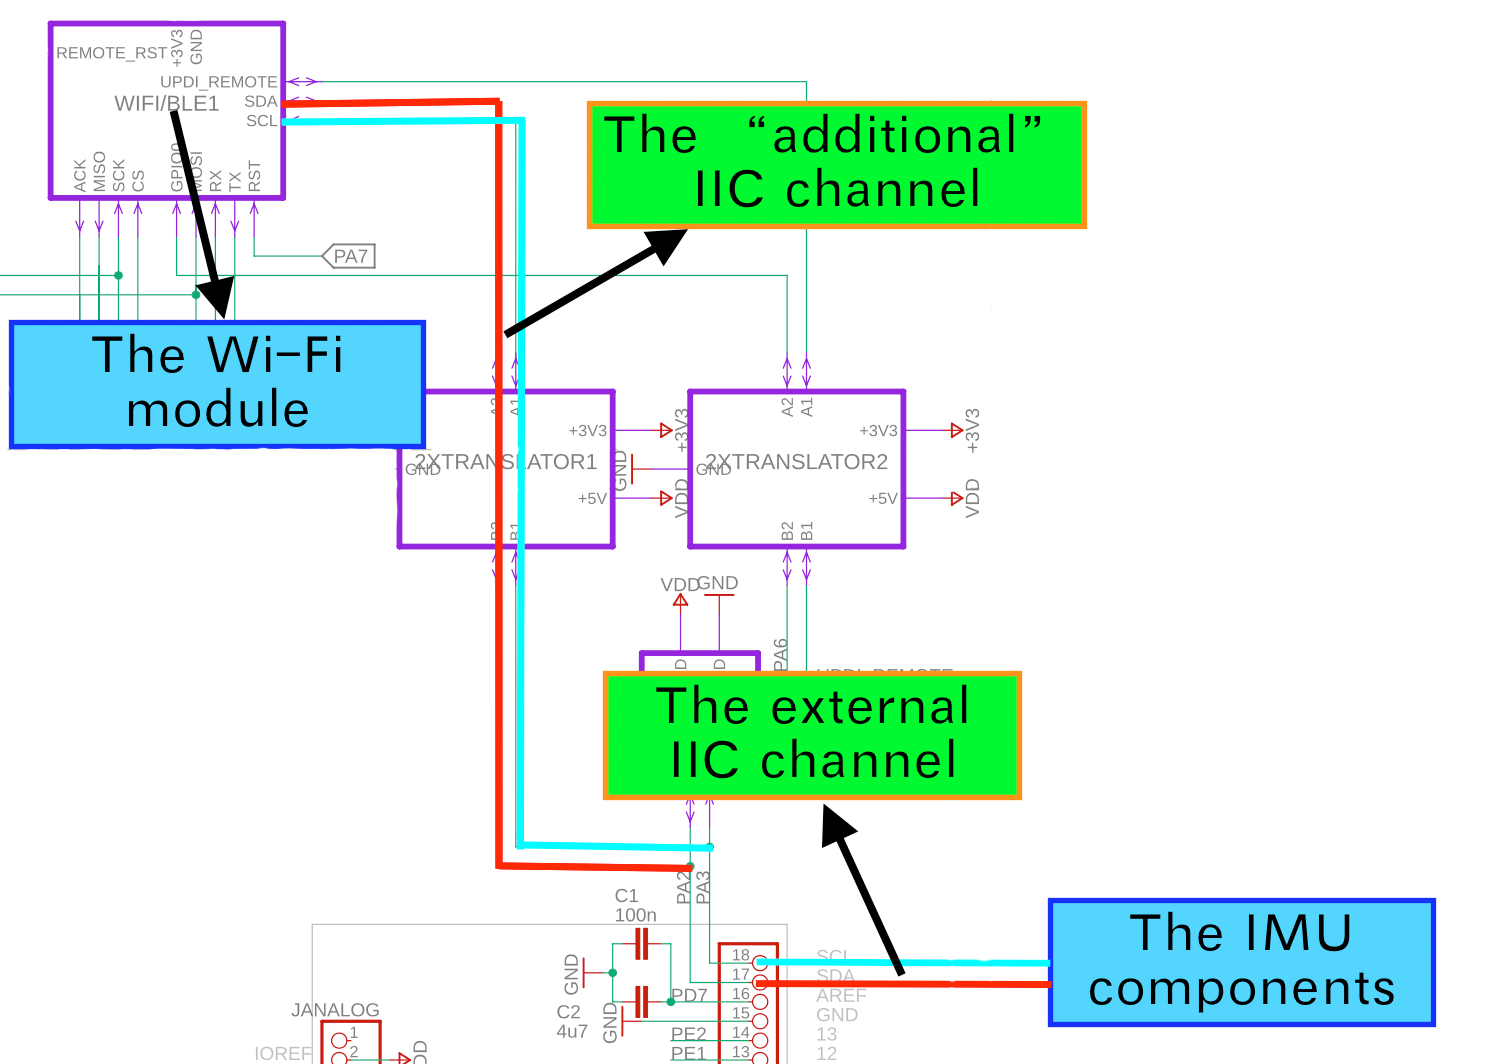
\includegraphics[width=0.8\textwidth]{
		fileForWriting/IIC-conflict}
	\caption[Schematic for the Arduino-UNO-Wifi-Rev2]{Partial schematic for the Arduino-UNO-Wifi-Rev2, where the MCU, Wi-Fi module, and IMUs are sharing a same I2C communication channel.
	}
	\label{fig:IIC-conflict}
\end{figure}
%--------End of this FIGURE -----------



Based on such troubleshooting, a hypothesis was formed that the external I2C might have an impact on the internal I2C, which could then result in a ``no socket available'' error in the Wi-Fi module.
Additionally, during testing, it was noticed that shaking the IMU could subsequently trigger the error.
It was speculated that the internal I2C requires a high level of communication quality.
Hence, one possible solution is improving the poor cables captured by the image of  Figure~\ref{fig:IIC-connections} (a).


\subsection{Problem solving}
\subsubsection{Improve IIC communication quality}

To prevent potential problems raised by poor IIC communication quality, a multicore screened cable was therefore applied, as Figure~\ref{fig:IIC-connections} (b) may show.
Successfully, the Arduino could now continuously send motion data to remote server.


\begin{figure}[htbp]
	\centering
	\begin{subfigure}[b]{0.45\textwidth}
		\centering
		\includegraphics[width=\textwidth]{fileForWriting/original-connection}
		\caption{Original connection using dupont line.}
	\end{subfigure}
	\hfill
	\begin{subfigure}[b]{0.45\textwidth}
		\centering
		\includegraphics[width=\textwidth]{fileForWriting/improved-connection}
		\caption{Improved connection using screened cable.}
	\end{subfigure}
	\caption[]{Two types of connections to build the external IIC channel.}
	\label{fig:IIC-connections}
\end{figure}

\subsubsection{Remove the ``additional'' IIC channel}
During the following week of testing, the issue did not reoccur.
However, after several accidental drops of the device, the problem resurfaced and the Arduino could not stably send motion data to server.

To solve the issue from root, the ``additional'' IIC channel was physically removed by desoldering two resistors on that channel as Figure~\ref{fig:remove-IIC} may show.
As expected, the Wi-Fi module was indeed functioning well without any interference from external IIC channel.
This success also proved the correctness of previous analysis.


In summary, the Wi-Fi module is very vulnerable to any external interference in its IIC channel.
If affected, it may stop working and throw a ``no socket available'' error.
As the MCU and module use another SPI channel to communicate, we decided to physically remove that IIC channel since this project did not require an IIC functionality of that module.
After the removal, the whole system worked perfectly.
The root of such issue may be the design flaw of Arduino-UNO-Wifi-Rev2, where the MCU, Wi-Fi module, and external IIC devices directly share one IIC channel.
Simultaneously, the Wi-Fi module may require a high level of communication quality.


%-----------This is a FIGURE-----------------------
\begin{figure}[htbp]
	\centering
	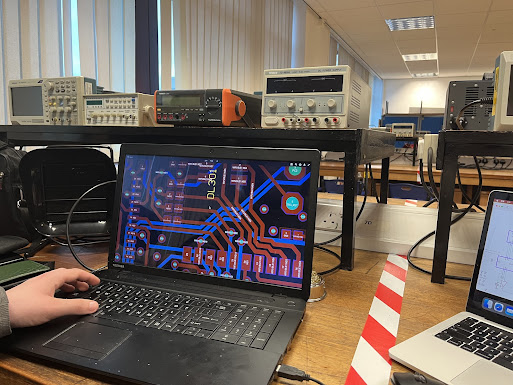
\includegraphics[width=0.7\textwidth]{
		fileForWriting/remove IIC}
	\caption{Desoldering two resistors on the ``additional'' IIC channel to completely solve the ``no socket available'' issue.}
	\label{fig:remove-IIC}
\end{figure}
%--------End of this FIGURE -----------







